% vim: ft=tex
\chapter{Methodology}
TODO what have we done to arrive at the goal (should be reproducible)\\
TODO this is probably what we know as "Concept"\\


\section{Getting Familiar with Roadster}
TODO: this is the first task according to Task Description\\
TODO andy's introduction during first Friday morning\\
TODO first impression of Roadster's code base: very clean, abstractions, loosely coupled, scarcely documented

\section{Testing}
Diese Section beschreibt die Testmethods welche wir angewandt haben, um die 
einzelnen Funktionen, das Zusammenspiel der Komponenten, sowie das Verhalten 
der Applikation als ganzes zu testen. Alle Resultate zu den Tests können im 
Results Kapitel entnommen werden.\\
\\
This section describes the test methods we used to check single functions, 
the components interaction and the behaviour of the whole application.
All resuts of the tests can be found in the results section.

\subsection{Setup}
Zur Umsetzung von Continous Integration wird gitlab CI verwendent, weil gitlab
kostenlos ist im gegensatz zu seinem pendant Travis CI, welches nach mehr als 100
Builds kostet bei privaten repositorys. 
Daher wurde gitlab CI auf dem HSR Server installiert und konfiguriert.\\
\\
Due to the fact that our repository is private, we can't use the online 
travis ci without to pay for it, because after 100 build it costs.
We had to install on our hsr server gitlab. Gitlab has a own continous integration 
which we used for unit and integration test. Each commit execute all unit tests and 
integration tests. This is straightforward to check if all components work together correctly.

\subsection{Unit test}
Um die Richtigkeit der Implementationen zu gewährleisten wurden Unittests mit
Ruby Unit gesetzt, welche die Kernfunktionen testen. Die Unit Tests sind im Source Code zu finden.\\
\\
To ensure the correctness of the implementations were ruby unit tests set 
which test the functions. Whenever the functionality of the application was changed or
a bug was fixed, new tests were added to cover the new behavior.
An other benefit of the tests was, we could refactoring the code and check 
if nothing on the behaviour changed.\\
For each commit to the repository every test has to pass otherwise it is
an offend against our team contract.\\
The unit tests can be found in the source code.

\subsection{Integration test}
Integration tests überprüfen das Zusammenspiel zwischen den einzelnen Komponenten.
Um unsere Kern Features zu testen (Cluster, HA, persistence) schreiben wir
integration tests mit ruby unit tests. Dazu starten wir jeden Node als eigenen Prozess.
ZMQ erlaubt es uns die "Inter-Kommunikation" auch über Prozesse zu testen.
Um Verbindungsprobleme zu testen werden die einzelnen Prozess "gekillt" um ein Failover zu erzwingen.\\
\\
Integration tests verify the interaction between the individual components. 
To test our core features (like cluster, high availability, persistence). We wrote integration
tests with ruby unit tests. To test the interaction between nodes, we started the roadster application
in different process. ZMQ allows us to interact between process and they will act like internode connections.
In order to test the failover or synchronization functionality the individual process - "node" 
can be killed and started again later if the scenario defines this.\\
\\
More detail about the integration tests scenarios can be found under the results chapter.

\subsection{Continous integration}
Continous Integration soll Aushilfe schaffen beim Elimnieren von Integration Problemen. 
Daher wird CI bei jedem Push ins Github Repository ausgeführt. Dazu überwacht gitlab 
das Repository und führt das definierte Build zum Projekt aus
Dieses Build beinhaltet das installieren von Abhängigkeiten, das Installieren der Roadster app und
zu guter letzt das Ausführen der Tests.\\
\\
Continous integration helps us to prevent integration problems also known as "integration hell". On
each push to the repository will trigger an CI check. Therefore gitlab hooks our repository and 
runs the defined build from the project. A Build containts the installation of the dependencies, 
installing the roadster app and the carrying out of tests.

\subsection{System test}
Systemtests dienen dazu die Applikation unter realen Bediengungen zu testen. Um eine fast realitätsnah
Umgebung zu erschaffen, kam mininet, jnettop und fake SPS Steuerungen zum Einsatz.
\begin{description}
	\item [Mininet:]
		Mininet erlaubt es adhoc VirtuelMachine's zu starten, 
		welche einen gemeinsamen Kernel teilen.
		Dies ermöglicht es auf einem Rechner viele Nodes/Rechner zu starten. 
		Mittels mininet können auch Verbindungen zwischen Nodes getrennt werden
		um Netzwerkprobleme zu simulieren. 
	\item [jnettop:]
		jnettop simuliert Netzkapazitätprobleme auf den einzelnen Verbindungen.
	\item [fake sps:]
		Fake SPS Steuerungen sind einfache Scripts, welche auf Anfragen antworten.
\end{description}

Alle Ereignise wurden in Logdateien gespeichert, welche für die Auswertung des Ergebnis gebraucht wurden. 
Mit einem Ruby Programm wurden diese Logdateien auf korrektheit überprüft.
Alle Systemtests wurden manuell nach jeder construction phase ausgeführt.\\
\\
System tests are designed to test the application under real conditions. 
To create an almost realistic environment we used mininet, jnettop and fake PLC controls for deployment.
\begin{description}
	\item [Mininet:]
		Mininet allows adhoc start VirtuelMachine's, which share a common kernel.
		This makes it possible on a computer to start many nodes / hosts. 
		Mininet can also simulated connection problems between nodes.
	\item [jnettop:]
		jnettop simulated network capacity problems on the individual network connections between the nodes.
	\item [fake sps:]
		Fake PLC controls are simple scripts that respond to requests.
\end{description}

All events were stored in log files, which were used for the evaluation of the result. 
A Ruby program checked these log files on correctness. All system tests were performed manually 
after each construction iteration.

\subsubsection{Test scenarios}
Die Testszenarien enthalten primär nur mögliche Bediengungen wie sie in einer realen Situation anzutreffen sind. Aus wissenschaftlichen Interesse wurden weitere Szenarien
getestet, welche den Extremfall abbilden sollten.\\
\\
The test scenarios only includes possible combinations as they are encountered in a real situation. From scientific interest
we added more test scenarios, which reflected the extreme cases.
\begin{description}
	\item [ML-HA:]
		Multi Layer mit zwei ebenen. Die erste Ebene enthält ein Node, 
		welches die Steuerungen überwacht. Die zweite Eben hat einen Primary und Backup.
	\\TODO ...
	\item [SL-HA:]
		Single Layer. Ein Primay und Backup Node welche beide direkt mit der Steuerungen verbunden sind.
		\\TODO ...
\end{description}
Persistence wird bei allen Tests mit geprüft, da sie zu Non functional requirements gehört und bei allen Szenarien aktiv ist.
\\TODO Extremfall ... 3 Ebenen mit 1 ebe
\\
Testszenarien enthalten die Konfiguration von Mininet und den einzelnen Nodes. 
Der Ablauf der Szenarios wurde im Detail beschrieben um die Ergebnisse reproduzierbar zu machen.


TODO work out methodology (maybe with mininet, shell scripts, and analyze logs retrospectively)\\
TODO integration tests at the end of every iteration\\
TODO system tests at end of construction\\
TODO use travis-ci.com OR GitLab CI (self-hosted on HSR VM)\\

%----------------------------------------------------------------------------
\section{Port to new \zmq library}\label{sec:meth:port}
TODO justify why port is needed right at the beginning (exclude faults from unmaintained ffi-rzmq gem, encryption is needed anyway, all the other tasks involve communication over ZMQ)\\
TODO explain binding options out there, why CZTop (including difference between ZMQ and CZMQ)\\
TODO explain preliminary task of adding support for the ZMQ options \sh{ZMQ_FD} and \sh{ZMQ_EVENTS} in CZTop\\
TODO explain concept of exchanging ffi-rzmq with CZTop\\


%----------------------------------------------------------------------------
\section{Cluster}\label{sec:meth:cluster}
TODO describe scribble (chp.pdf)


\subsection{Aspects}
Adding cluster functionality to Roadster involves the following aspects:
\begin{itemize}
	\item node topology DSL

		This DSL also has to provide means to define the roles/functionality of each node, e.g. the set of COMM actors running on a particular node

	\item DIM synchronization
	\item message routing
	\item What needs to be done if a WebUI user wants to e.g. change some value on a PLC, possibly on a remote node? Is it completely handled via DIM or do we need message routing?
\end{itemize}

\subsection{DIM Synchronization}
TODO election/design of appropriate protocol\\

\subsubsection{The Existing CSP in a Nutshell}
\emph{This is a brief introduction/refresher for the Clone State Pattern
implemented by Roadster. Although Roadster actually sends serialized instances
of CSP message classes to fulfill this protocol, for better readability the
Zguide's canonical nomenclature of Clone Pattern messages will be used.}

The existing CSP is closely related to the Clone Pattern from the Zguide\footnote{\url{FIXME}}. Its
goal is to keep a state (a list of key-value pairs) in sync across a set of
participants. To greatly reduce the complexity, it's not decentralized: There's
a server part which serves as the single source of truth.

The server uses a ROUTER, a PULL, and a PUB socket; each client a DEALER, a
PUSH, and a SUB socket. The protocol consists of three distinct messages flows:

\begin{description}
	\item [Snapshots:]
		Requesting and receiving the complete, current snapshot of the
		state (all key-value pairs). This happens via a
		ROUTER/DEALER pair of sockets. The request message consists solely of
		the humorously named ICANHAZ command. The response is the
		complete set of KVSET messages so a late-joining (or previously
		disconnected) client can rebuild the current snapshot.

	\item [Upstream updates:]
		Updates always originate from clients and are sent to the
		server via a PUSH/PULL pair of sockets. These are KVSET messages.

	\item [Downstream updates:]
		After being applied to the server's copy of the state,
		updates get a sequence number and are published back to all
		clients. This happens via the PUB socket and
		uses KVPUB messages.
\end{description}

By making all updates go through the server, a total order is enforced,
which is crucial to keep the state consistent across all clients.

To avoid risking a gap between requesting the current snapshot and subscribing
to updates, a client actually subscribes to the updates first, then gets the
snapshot, and then starts reading the updates from the socket (which has been
queueing updates in the meantime, if any). Updates that are older or the same
age as the received snapshot are skipped, and only successive updates are
applied (tested by comparing the sequence numbers).

Because message loss via the third message flow (PUB-SUB) is unlikely but
theoretically possible, the client checks for gaps in the sequence number of
each KVPUB message. If a gap is detected, the current state is discarded and a
complete resynchronization happens. This is brutal, but is very simple and thus
robust; there's no complexity that would leave room for nasty corner cases.

Keys can be treated hierarchically (e.g. \sh{topic.subtopic.key}) and thus, a
client can optionally subscribe to only a particular subtree. This is useful
when the number of client grows and not all of the state needs to be on every
client. In that case, the topic of interest is sent by the client along with
the ICANHAZ message.

\subsubsection{What's Missing}
TODO it has to work across several nodes\\
TODO it has to be able to handle HA supernodes\\
TODO explain Clustered Hashmap Protocol (?)\\
TODO PCP: use DIM to know node tree and determine next hop for (dialog or fire+forget) messages
TODO mention CAP theorem, we need AP since sub trees are autonomous, but we guarantee eventual consistency by restricting write access to the owning node\\

Here are the possible variants:

\begin{description}
	\item [Variant 1. Sync self-subtree only:] \hfill
		\begin{itemize}
			\item always sync on self-subtree only
			\item con: no copy of remaining tree
		\end{itemize}

	\item [Variant 2. Sync complete tree:] \hfill
		\begin{itemize}
			\item always sync on complete tree
			\item get snapshot and merge own subtree
		\end{itemize}

	\item [Variant 3. Either sync on subtree or complete tree:] \hfill
		\begin{itemize}
			\item make it configurable: either sync on subtree or complete tree
		\end{itemize}
\end{description}

Variant 2 will be the first step. Variant 3 will be the second step, if at all.


\subsubsection{What's needed}
Since COMM actors are used to communicate with the outside world, new COMM
actors will have to be introduced: One kind that is south-facing to communicate
with subnodes, and another one that is north-facing for communication with
supernodes. We'll call them COMM CLUSTER NORTH and COMM CLUSTER SOUTH.

Their responsibility is the inter-node synchronization of the DIM, similarly to
what's happening in the existing CSP within a single node.

\begin{itemize}
	\item they do something closely related to the existing CSP
	\item future oriented: because of the HA requirement, ideas from the CHP are integrated, such as using PUB-SUB (instead of PUSH-PULL) for inter-node KVSET messages, so both super nodes (in HA setup) hear updates
	\item for intra-node KVSET messages, PUSH-PULL is OK and can be left unchanged
	\item only node A has write access to values on A (to avoid uncertain situations involving race conditions), e.g.:
\end{itemize}

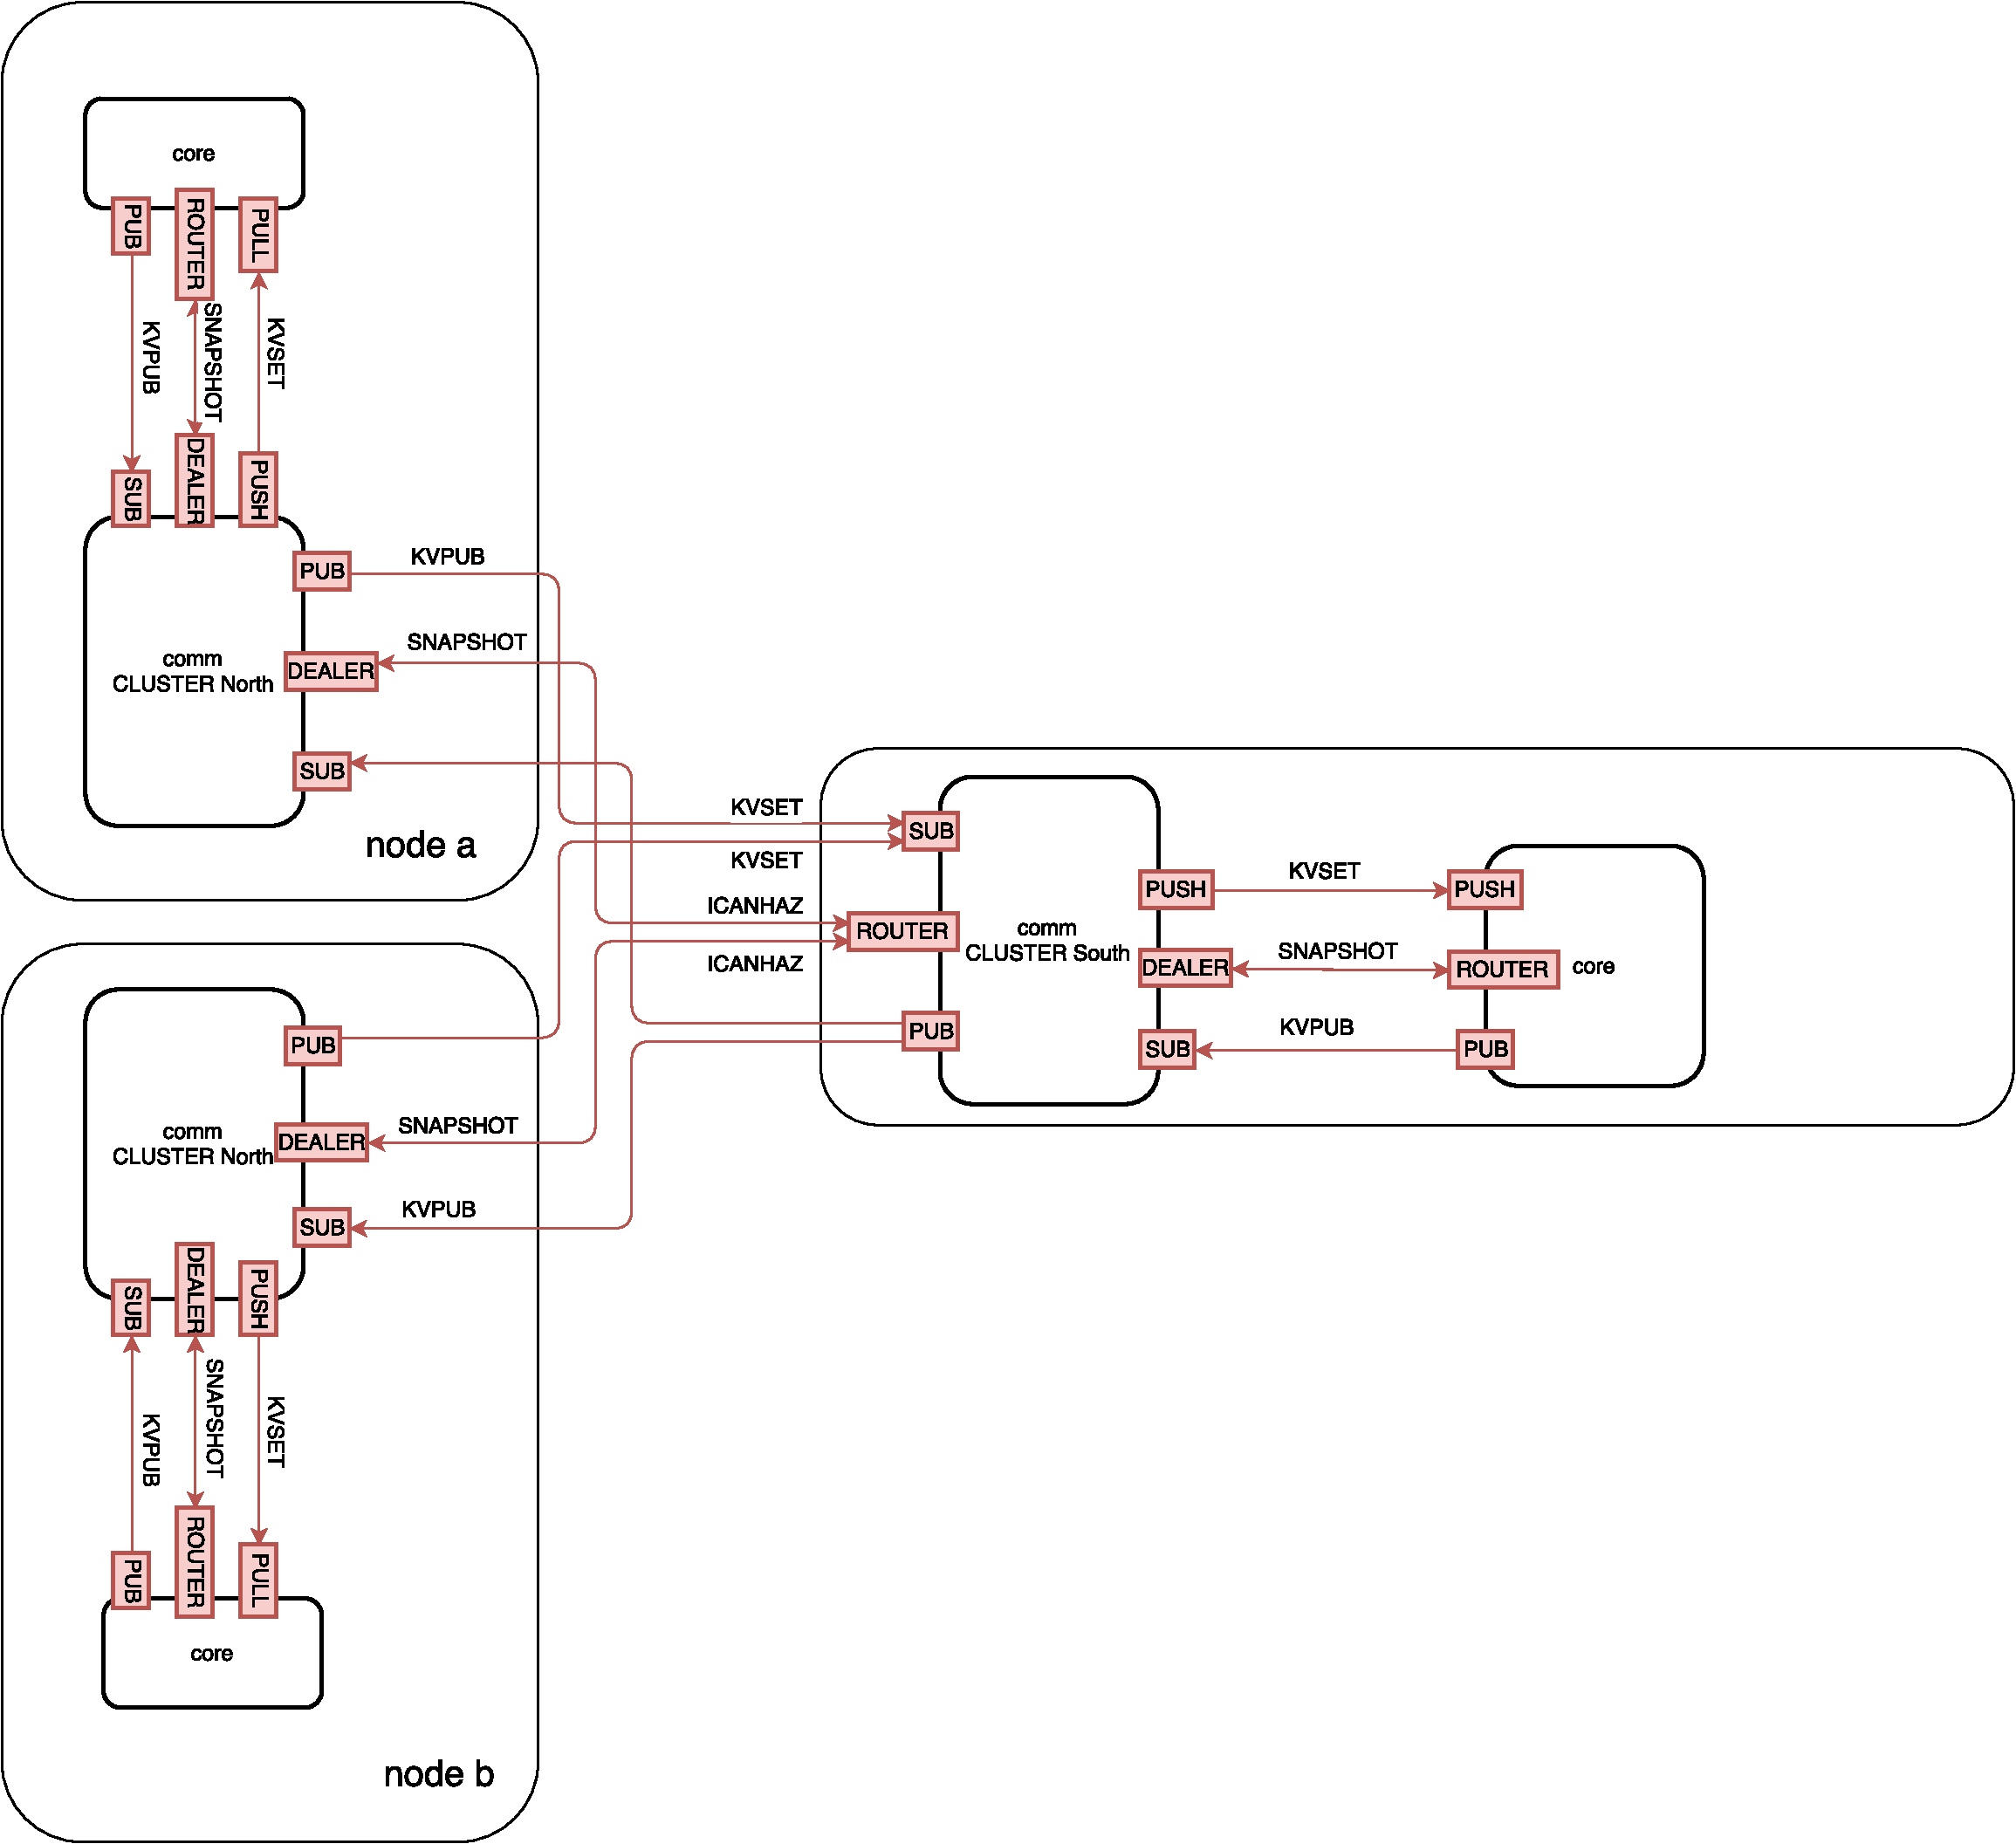
\includegraphics[width=\textwidth]{img/cluster_protocol.pdf}

\subsection{Node Typology Definition}

\begin{itemize}
	\item node topology in DSL, static file (e.g. topology\_conf.rb) shared on all nodes, read by each actor on startup
	\item specific config file on each node (conf.rb) knows its own place in topology (through \rb{conf.system_id})
	\item maybe a HA pair is one DIM object, has one name, but two IP addresses (primary and backup, in order)
\end{itemize}

\begin{lstlisting}[style=customruby]
# * basic method to add a node: #add_node(ID, south_facing_bind_endpoint)
# * it takes a block for defining subnodes

##################
# without HA:

conf.nodes do |map|
  map.add_node("root", "tcp://10.0.0.1:5000") do |map|
    map.add_node("subnode_a", "tcp://10.0.0.10:5000")
    map.add_node("subnode_b", "tcp://10.0.0.11:5000")
  end
end

# subnode_a can infer its endpoints from its position in the tree:
conf.system_id = "nodes.root.subnode_a"
#=> this node is "subnode_a"
#=> its IP address is 10.0.0.10
#=> north facing COMM actor's bind port is 5001
#=> south facing COMM actor's bind port is 5000
#=> north facing COMM actor will connect to "root" node on "tcp://10.0.0.1:5000"

#####################
# later with HA:

conf.nodes do |map|
  map.add_ha_pair("root", "tcp://10.0.0.1:5000", "tcp://10.0.0.2:5000") do |map|
    map.add_node("subnode_a", "tcp://10.0.0.10:5000")
    map.add_node("subnode_b", "tcp://10.0.0.11:5000")
  end
end

# subnodeA can infer its endpoints from its position in the tree:
conf.system_id = "nodes.root.subnode_a"
#=> this node is "subnode_a"
#=> its IP address is 10.0.0.10
#=> north facing COMM actor's bind port is 5001
#=> south facing COMM actor's bind port is 5000
#=> north facing COMM actor will connect to "root" HA pair on "tcp://10.0.0.1:5000" OR "tcp://10.0.0.2:5000" (Lazy Pirate algorithm)

# for primary root:
conf.system_id = "nodes.root[primary]"

############
# within ba-roadster-app's lib/domain/domain.rb file:
#
# Idea for node topology definition and assigning roles (features/adapters) to
# diffent kinds of nodes.

module Roadster
  module Domain::Model

    build do
      nodes do
        node "root" do # or maybe ha_node or bstar_node
          endpoint "tcp://10.0.0.1:5000", "tcp://10.0.0.2:5000"
          label 'BA Roadster App'
          desc  'Sample application for experimenting and developing the new features within the scope of the Bacherlor Thesis of Patrik Wenger and Manuel Schuler at HSR.'

          load_conf ::Conf::AccessControl
          load_conf ::Conf::Objects
          load_conf ::Conf::Navigation

          node "subnode_a" do
            endpoint "tcp://10.0.0.1:5000"
            load_conf ::Conf::Adapters
            # load_conf ...
          end
        end
    end

  end # Domain::Model
end # Roadster
\end{lstlisting}


\subsection{Message Routing}
TODO message routing (end-to-end routing with identity/identities as prepended message frame?, should be simpler and more efficient than hop-by-hop routing)\\

%----------------------------------------------------------------------------
\section{High Availability}\label{sec:meth:ha}
If Roadster is going to be run in a cluster setup, measures need to be taken to
mitigate the risk of failure, since many nodes are more likely to fail than a
single node (unless they add redundancy). Availability shall be ensured by
adding redundancy on certain levels of the node hierarchy (e.g. at the bottom
of the topology, right above the PLC, or at the root level), in the form of a
fully functional backup node in addition to the primary one.

Run together in a hot-standby cluster, the passive node's responsibility is to
take over in case the active one goes down.

\subsection{Defining Reliability}
When speaking about reliability, it's worth listing the failures we want to be
able to handle. According to the requirements, these are exactly:

\begin{description}
	\item [Hardware or software failure on the primary node:]
		This could be one of the actors crashing, the whole OS
		crashing, or a fatal disk failure, irrecoverable memory error,
		or even just someone accidentally pulling the power plug.

	\item [Network failure]
		This only includes the failure of the link between the two HA
		peers. Interestingly, this limitation applies to both single
		level and multi level HA.
\end{description}


Failures that won't be covered include:
\begin{description}
	\item [Failure of the link between a subnode one of the supernodes:]

		This can't be handled since the two HA peers would have to
		continually share the number of subnodes connected to them, and
		based on that, make a decision on which one should be active or
		passive. Since the link between them could fail as well, this
		decision can't be done reliably, which could lead to the
		dreaded split brain syndrome.

	\item [Failure of the link between a HA peer node and the PLC]
		The Binary Star alrogrithm won't initiate a failover since the
		active is still alive and is able to tell the passive node so.
		The missing life signs via the PLC could cause an alarm, but no
		failover, since they're only half of the conditions that have
		to be met for a failover.
\end{description}

\subsection{What's Needed}
TODO A simple HA protocol => Binary Star\\
TODO maybe we need to extend binary star to handle other kinds of network failures?\\
TODO new actor: COMM BSTAR\\

\subsection{Binary Star in a Nutshell}
TODO explain binary star\\
TODO two conditions (no heartbeats, and vote)\\

\subsection{Failover}
In case the currently active node goes down, the two conditions will be met.
This means that the passive node starts accepting snapshot requests (ICANHAZ
messages) and updates the DIM, so every other node will know about the new,
active node. This is needed for the message routing to work.

\subsubsection{Alarm Generation}
When a failover happens, we want to create a \rb{Case} (alarm) in the DIM, so
the outage is visible to a user in one of the web UIs. Also, in case the
passive node goes down, which doesn't have an immediate effect on availability,
we also want to create a \rb{Case}. This is so the user can act upon the alarm
and e.g. initiate field forces to inspect the failed node and repair it.

Once repaired, it's started with the exact same configuration (either primary
or backup) again. Since there's already an active node (either the primary one,
or the backup one), the newly repaired node will become the new passive node.

\subsubsection{Failover from Backup to Primary}
Once failed over, the newly actve backup node stays active. It does so until it
fails itself, at which point the now repaired, up and running primary node will
take over. This works because the Binary Star protocol operates symmetrically
after successful initialization. But it never automatically switches back to
make the primary node the new active one without a failure. This is key. If a
node goes down, the failover happens automatically, but anything else will
require human interaction.

\subsection{Side benefit: Rolling Upgrades}
TODO useful for upgrades (maybe in Discussion)\\

\subsection{Single Level}
This is different from what's described in the zguide because the concept of
client requests is missing here (PLCs don't request anything).  What can be
done instead is periodically sending life signs from one node to the other
through the PLC by updating some designated memory block. This can actually be
done by both the active and the passive node, which reduces code complexity.

The passive node will check the active node's life signs periodically as well.
In case the life signs cease, it can give its vote to the COMM BSTAR actor.
This would satisfy the second condition of the Binary Star protocol for a
failover to take place. The first condition would be the missing heartbeats
which are normally transmitted through the network link.

TODO new actor: COMM PLCVOTER\\

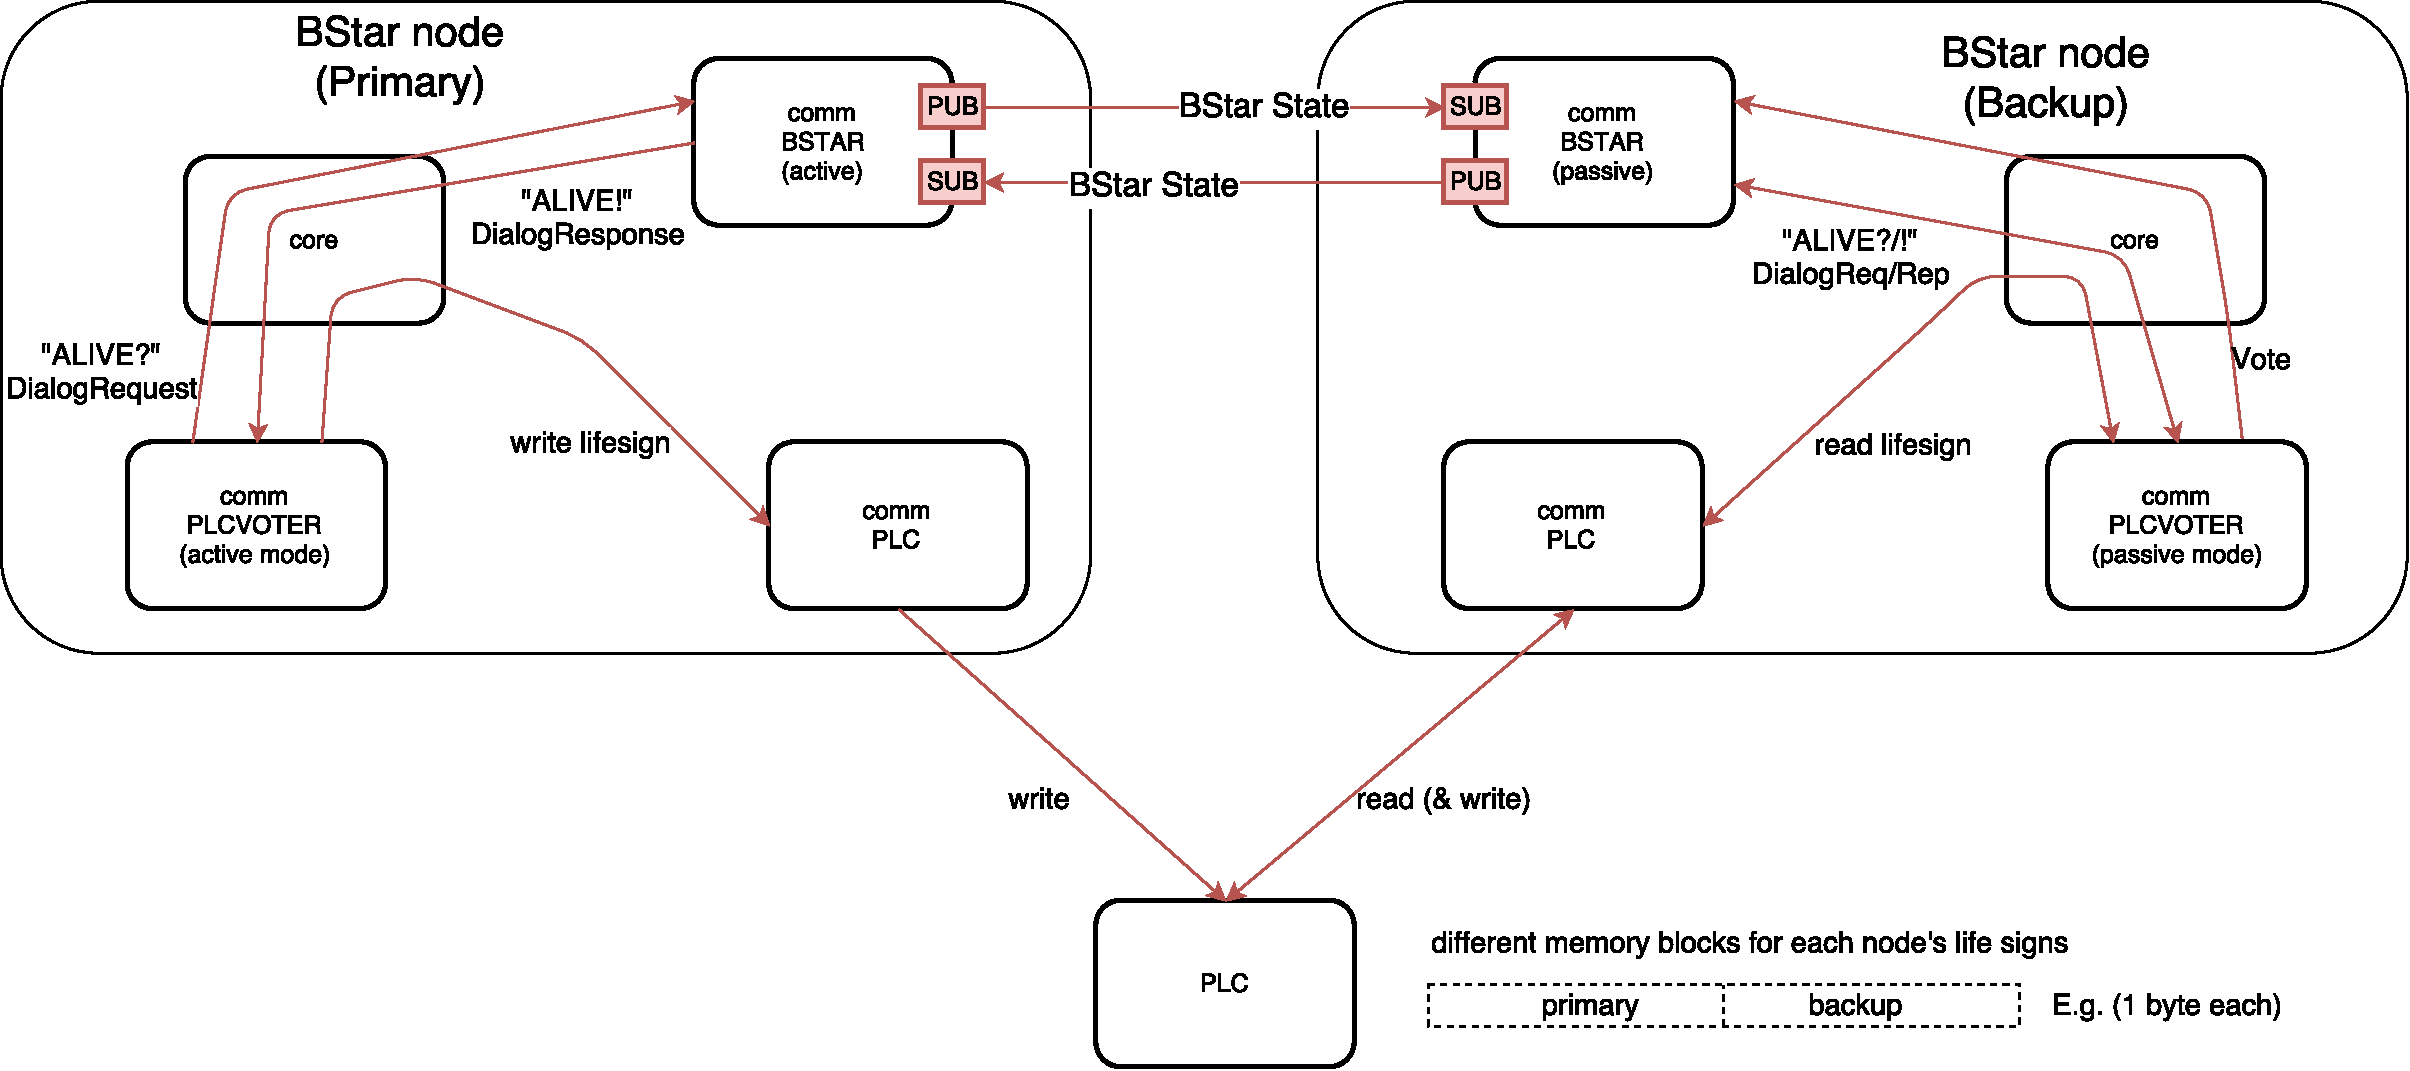
\includegraphics[width=\textwidth]{img/SL-HA_bstar.pdf}

\subsubsection{Caveats}
Special attention needs to be paid when it comes to writing these life signs. A
na\"ive developer might implement the COMM PLCVOTER so it autonomously causes
life signs to be written PLC. This works as long as the failures only affect
the hardware. But what if a software error happens in the CORE or BSTAR actor?
They'd crash or hang, while the PLCVOTER happily sends out life signs, which it
obviously shouldn't be doing at that moment.

A better implementation would have the PLCVOTER poll the BSTAR via the CORE
router whether it's still alive, and only send out a life sign in case it gets
an answer. This way, the BSTAR and the CORE actor are being tested for
responsiveness. We'll call the two messages being sent back and forth "DEAD?"
and "ALIVE!".

\subsubsection{Node---PLC Link Failure}
TODO describe why this won't cause a failover and thus can't be handled, as
mentioned above\\

\subsubsection{Supporting Different PLCs}
TODO: adapter

\subsection{Multi Level}
This kind of HA setup is closely related to the Binary Star Pattern described
in the zguide, meaning that there will be actual requests from client on the
passive node in case the active node fails. These requests will count as votes
to fulfill the second condition that has to be met for a failover to be
initiated.

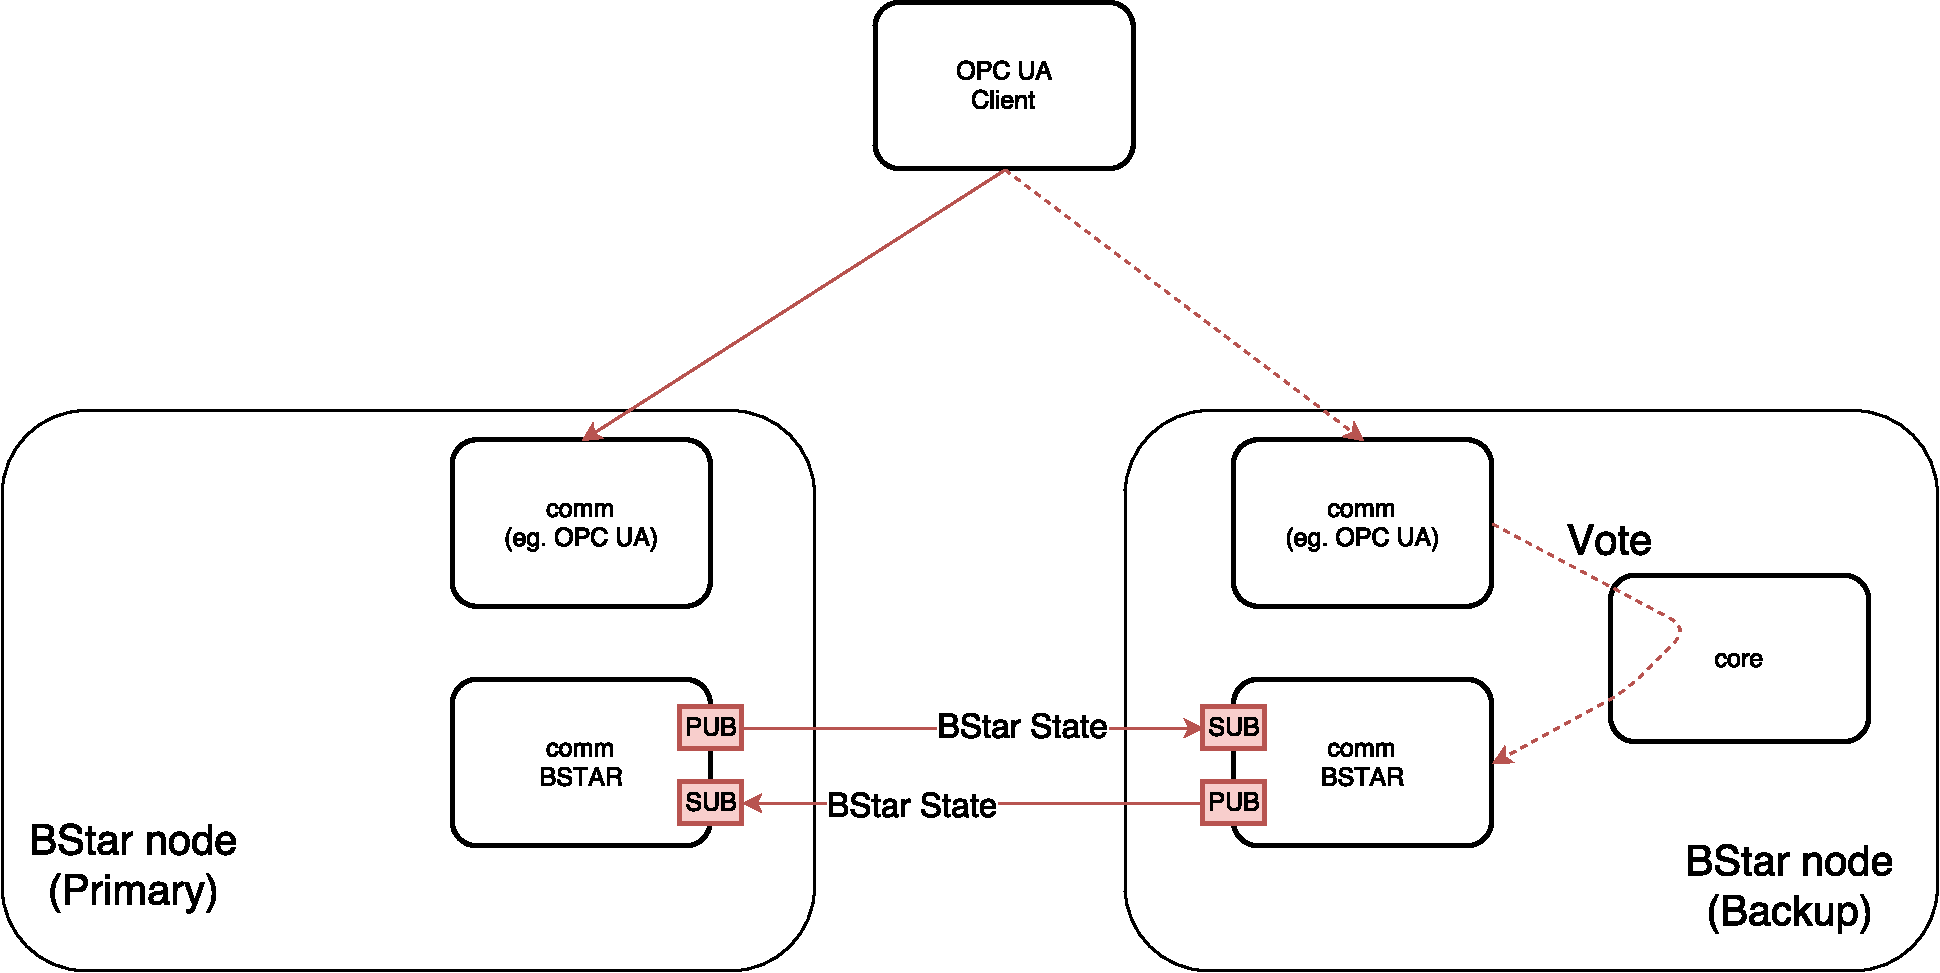
\includegraphics[width=\textwidth]{img/ML-HA_bstar.pdf}

%----------------------------------------------------------------------------
\section{Persistence Synchronization}\label{sec:meth:psync}
The persisted data needs to be bubbled up towards the root node.

\subsection{Aspects}
There are multiple aspects involved in persistence synchronization:

\begin{description}
	\item [Delta:]
		How does one get the initial delta of updates since last
		synchronization?

	\item [Updates:]
		Further updates, one-by-one. This is only needed in
		case the solution aims for real-time synchronization.

	\item [HA peer sync:]
		How does the inactive HA peer get updated? Of
		course, this only matters when the supernode is HA pair.
\end{description}

\subsection{Variants}
There are multiple variants to achieve the needed functionality.

\subsubsection{Polling only}
The supernode just periodically request persistence
deltas. This would be handled over a DEALER/ROUTER pair of sockets. The nice
thing about this variant is that the subnode only has to do one thing, which is
responding to requests from the supernode(s); it doesn't have to proactively
send any updates after sending the an initial delta.

A big drawback is that the synchronization doesn't happen in real-time. This
doesn't seem to fit well into the overall Roadster architecture, which is
completely event-driven (no polls or "sleeps").

TODO another drawback: computing the diff might be heavy (depending on DB)

In case the supernode is a HA pair, this variant would generate duplicated
traffic. To avoid this, another pair of sockets has to be introduced to
synchronize persistence between a HA pair. This also means designing another
protocol, and more moving parts overall.

Overall, this variant is very simple, but doesn't offer some features we'd
normally expect from a framework like Roadster. The fruits are hanging low;
achieving real-time synchronization is easy.

\subsubsection{PUSH-PULL}
This variant avoids the delays introduced by the polling mechanism of the first variant.

Procedure (for each subnode):
\begin{enumerate}
	\item via a ROUTER/DEALER socket pair:
		\begin{enumerate}
			\item supernode tells subnode its most recent timestamp in an ICANHAZ request
			\item subnode sends delta
			\item supernode receives and processes the complete delta
		\end{enumerate}
	\item subnode sends updates to supernode via PUSH-PULL
	\item during low-traffic times, we can send HUGZ as heartbeats
\end{enumerate}

This seems nice at first, but PUSH socket's send buffer will fill up when the
connection is interrupted.  This isn't bad in and of itself, because when it's
full (and writes start to block), we can just destroy the socket and
reinitialize and start syncing anew (from ICANHAZ) after a certain timeout.
But the problem is that, in case the delta is large, it will inevitably fill
the PUSH socket's send buffer, temporarily reaching its high water mark, which
is part of its normal operation.

So we'd have to introduce logic to recognize whether the PUSH
socket is just temporarily full (e.g. during delta transmission), or
permanently full (e.g. the supernode or the link to it is down).

Another disadvantage is that there needs to be another channel to synchronize
persistence updates to the other HA peer, if there is one. This means another
pair of sockets, another protocol to be designed, and more moving parts
overall.

\subsubsection{PUB/SUB}
This is similar to CSP/CHP. It's not 100\% reliable, but even with unstable
links, no data loss will occur if the client (the supernode) is able to reconnect within a
specific amount of time. \zmq's default for that amount is 10 seconds. As the
requirements specify, 100\% consistency is not mandatory for the persistent
data.

A possible drawback is that the traffic is duplicated in case the supernode
is a HA pair. However, there are numerous opportunities to mitigate this.

Procedure (for each subnode):
\begin{enumerate}
	\item supernode subscribes to updates from subnode
	\item via a ROUTER/DEALER socket pair:
		\begin{enumerate}
			\item supernode tells subnode its most recent timestamp in an ICANHAZ request
			\item subnode sends delta
			\item supernode receives and processes the complete delta
		\end{enumerate}
	\item supernode starts reading updates, possibly skipping the first few (based on timestamp)
\end{enumerate}

\subsection{Chosen Variant}
We'll most likely go with the PUB-SUB variant, since it's simple and is similar to
what's used for the new CSP in conjunction with multi-node HA. It provides the best
opportunities to improve efficiency later on.

Its possible performance issues can be ignored right now, as trying to fix them
is arguably considered premature optimization. If this turns out to be an issue
in a productive deployment, like over a cellular network link, a future version
can switch to multicast. \zmq supports PGM, which is a reliable multicast
protocol. (Pragmatic General Multicast, standardized, directly on top of IP,
requires access to raw sockets and thus may require additional privileges) and
EPGM (Encapsulated Pragmatic General Multicast, encapsulated in a series of UDP
datagrams, doesn't require additional privileges, useful in a \zmq-only setup).

If its reliablity turn out to be an issue, one the socket option
\sh{ZMQ_RECOVERY_IVL} can be increased from 10 seconds to, say, 60 seconds, which
gives an unstable link more time to recover before any data loss happens.

TODO: describe reasonable default setting, in case we change ZMQ's default.


\section{Security}\label{sec:meth:security}
TODO This is the optional goal.\\
TODO briefly describe \zmq's security features, what's left for us to decide (key destribution, if at all)\\
TODO how it can be verified (-> using wireshark)\\
TODO why curvezmq is awesome (confidentiality, integrity, availability (server keeps no state until client is fully authenticated)




\section{OPC UA Interface: High Availability}\label{sec:meth:opc-ua}
TODO This is the optional goal.\\
TODO explain new opportunity for OPC UA HA server\\
TODO describe whatever needs to be described\\

\begin{itemize}
	\item study standard
	\item use Andy's gem
	\item according to Andy, this should be a simple thing
\end{itemize}
